\documentclass {report}
\usepackage{graphicx}
\usepackage{minted}
\usepackage{titlepic}
%\usepackage[romanian]{babel}
\usepackage{fontspec}

% To draw diagrams.
\usepackage{tikz}
\usepackage{float}
\usetikzlibrary{positioning, arrows.meta}
\usetikzlibrary{fit} % To merge nodes.

%\usepackage[utf8x]{inputec}
\usepackage{color}   %May be necessary if you want to color links
\usepackage{hyperref}
\setmainfont[ItalicFont={timesi.ttf},
						BoldItalicFont={timesbd.ttf}]{times.ttf}
\definecolor{light_blue}{RGB}{212,235,242}

% Edit table of contents links.
\hypersetup{
    colorlinks=true,  %set true if you want colored links
    linktoc=all,      %set to all if you want both sections and subsections linked
    linkcolor=black,  %choose some color if you want links to stand out
}

\title {Relatório Programação de II}

\titlepic{\includegraphics[width=\textwidth]{"game life.png"}}
\author{
  David Marinho\\
  \texttt{54560}
  \and
  Axel Amoroso Carapinha\\
  \texttt{55248}
}

\begin {document}
\date{}
\begin{figure}[t]
	\vspace {-2cm}
	\centering
	
\includegraphics[width=0.4\textwidth]{uni_logo.png}
\end{figure}
\maketitle

\renewcommand{\thesection}{\arabic{section}}
\makeatother

\tableofcontents 
\newpage

\section{Abstract}
	Este trabalho teve como principal objetivo usar Java e o paradigma da 
	programação orientada a objetos (POO) 
	para recriar as regras de uma versão do jogo da vida (de John Conway) 
	com cenouras, coelhos e ervas,
	sendo usada a biblioteca AWT e a framework Swing, ambas de Java, 
	para mostrar os resultados.

\section{Resumo do projeto}
	O principal objetivo deste projeto foi preencher um prado verde retangular 
	com coelhos e cenouras nas células indexadas, também retangulares.\\
	O prado tem extremidades adjacentes, como num toro topológico.\\
	As (no fundo únicas) entidades deste prado interagem entre si através das 
	regras aplicadas, podendo nascer, sobreviver, morrer e, apenas no caso 
	dos coelhos, passar fome.\\
	Assim, cada prado é definido pelo tamanho, pela posição inicial dos coelhos,
	pelas cenouras e pelo tempo de fome \textit{starveTime}, que define quanto 
	tempo os coelhos sobrevivem sem comer cenouras.\\
	Tal como no jogo da vida de John Conway, diferentes ajustes nestas definições 
	do prado geram resultados variadíssimos, e padrões complexos podem surgir 
	de regras tão básicas como as utilizadas, e resumidas em \textit{timeStep()}: 
	o mais importante método de instância de cada objeto da classe \textit{Grassland}.

\section{Introdução}
	O objetivo deste relatório é mostrar a estrutura do programa, 
	além de explicar com mais detalhe pormenores de implementação e 
	resumir os resultados.\\

\section{Desenvolvimento}
	\subsection{Decisões de implementação}
	\begin{itemize}
		\renewcommand\labelitemi{--}
		\item Foi usado apenas um array bidimensional.
		\item Cada entidade tem um ID, que no fundo serve para identificar a classe,
					o que permite uma conexão facilitada com o ficheiro 
					\textit{Simulation.java}. Acaba por ser a utilização das constantes 
					inteiras de classe GRASS, RABBIT e CARROT.\\
					Por conta disso, \textit{cellContents()} retorna o ID do objeto 
					retornado pelo método \textit{getCell()} que retorna o endereço 
					da entidade guardado no array do prado instanciado.
		\item O método de instância \textit{startGrasslandLife()} contém código 
					comentado que se mostrou notoriamente útil na verificação das 
					regras deste projeto e uma lógica com o mesmo intuito da presente 
					no ficheiro \textit{Simulation.java}: preencher o prado 
					aleatoriamente.
		\item Foram mantidos muitos métodos de instância com o modificador \textit{public} 
					para serem acedidos pelo ficheiro \textit{Simulation.java}. Os únicos 
					métodos privados estão relacionados com implementações das regras e 
					cálculos auxiliares para as mesmas.
		\item Foi alterada a ordem de utilização dos argumentos dos métodos que 
					acedem ao array devido a preferirmos uma interpretação diferente de 
					posições no array (linha (\textit{row}) e coluna (\textit{column})),
					mas mantendo a compatibilidade com a interpretação presente no 
					ficheiro \textit{Simulation.java} (\textit{x}, \textit{y}).
		\item Foi criada uma classe própria para excepções relacionadas com a 
					ausência de coelhos no prado, para alertar o utilizador de situações 
					que poderiam parecer estranhas, e para conseguir implementar mais 
					partes da matéria lecionada, outro dos objetivos deste projeto.
		\item Utilizou-se uma JFrame em vez de uma Frame, por ser mais leve em 
					termos de utilização de recursos e por possuir mais funcionalidades.
	\end{itemize}	

	\subsection{Principais dificuldades}
		Em primeiro lugar, surgiu uma dúvida: seria melhor usarmos um array 
		intermediário ou instanciar e alterar diretamente o novo Grassland?

		Por um lado, a primeira opção parecia adequada quando foi primeiramente 
		implementada: teriamos o 'meadowArr', uma variável de instância (um array) 
		do atual Grassland no qual as regras eram baseadas, e o 'newMeadowArr', 
		também variável de instância, mas esta última para se escreverem os resultados 
		da aplicação dessas mesmas regras.

		Mas isso originou vários problemas. Com essa implementação faria falta 
		copiar os dados desse 'newMeadowArr' para o \textit{Grassland} instanciado, 
		que à parte de \underline{ineficiente}, seria \underline{menos prático}. 
		Além disso, \underline{tornou-se mais complicada a sincronização dos dados}, 
		devido à desnecessaria complexidade da lógica. 
		E ainda, como todos os objetos instanciados referenciavam o seguinte objeto, 
		preocupou-nos que o \textit{garbage collector} do Java
		não considerasse o espaço ocupado por prados inutilizados (e por todas as 
		entidades nele criadas, que são mais espaço que referencia) como livre. 
		Isso não só seria um grave problema de memória, como vai contra a natureza do 
		objetivo do próprio programa, pois resultados complexos começam a surgir 
		após um certo número de iterações, e não deve ser um problema de memória a 
		definir quando é que a simulação deveria parar.

		Por outro lado, o modo, implementado e mais prático, foi instanciar o 
		novo Grassland através do atual, 
		o que se provou útil em todas as fases do desenvolvimento deste trabalho.\\

		Em segundo e último lugar, surgiu a leitura diferente dos dados por parte do 
		método \textit{printGrassland()} e do ficheiro \textit{Simulation.java}
		
		Então decidimos fazer da seguinte forma para termos a certeza que os 
		Grasslands anteriores são limpos pelo GarbageCollector.

		\begin{minted}[autogobble, tabsize=2, obeytabs]{java}
			public Grassland timeStep() {
				Grassland newGrassland = new Grassland(this.width, this.height, this.starveTime);
					for (int row = 0; row < this.height; row++) {
						for (int column = 0; column < this.width; column++) {
							// Atualização do novo Grassland depois do atual ter passado pelas regras.
						}
					}
				 
				// Retornamos um novo Grassland.
				return newGrassland;
			}
		\end{minted}

\section{Procedimentos}
\begin{enumerate}
  \item Na execução do programa podem ser passados quatro argumentos por uma JFrame
				através de quatro objetos 'JTextField'.
		\begin{itemize}
			\item width \(\rightarrow\) O comprimento do prado.
			\item height \(\rightarrow\) A largura do prado. 
			\item starveTime \(\rightarrow\) Número de timesteps a que os coelhos 
					  sobrevivem sem comer qualquer cenoura. 
			\item maxTime \(\rightarrow\) Número máximo de gerações simuladas.
		\end{itemize}
	\item Um prado de comprimento i x j é preenchido com objetos do tipo 'Grass'
				e são gerados aleatoriamente outros objetos, objetos de tipo 'Rabbit' e 
				'Carrot'.
	\item A cada timestep é gerado um novo prado respeitando as regras a que
				a geração anterior esteve sujeita.
\end{enumerate}

\section{Design Patterns}
	Recorremos aos três pilares da Programação Orientada a Objetos (encapsulamento 
	herança e polimorfismo) criámos quatro classes para representar entidades
	específicas:
	\begin{itemize}
		\item	LifeBeing \(\rightarrow\) Classe mãe e abstrata das classes 'Rabbit',
					'Carrot' e 'Grass'.
		\item	Rabbit \(\rightarrow\) Classe filha que herda 'LifeBeing'. Tem como função 
					organizar todos os dados a respeito dos coelhos.
		\item	Carrot \(\rightarrow\) Classe filha que herda 'LifeBeing'. Organiza 
					toda a estrutura de dados a respeito das cenouras.
		\item	Grass \(\rightarrow\) Classe filha que herda 'LifeBeing' e organiza 
					toda a estrutura de dados a respeitos das ervas.
		\item Grassland \(\rightarrow\) Classe responsável por organizar todos os
					dados a respeito do campo, marioritariamente a posição dos objetos
					no campo e o tempo de longevidade dos mesmos. Mantiveram-se as 
					assinaturas dos métodos presentes na implementação base 
					de \textit{Grassland.java}
		\item Simulation \(\rightarrow\) Classe responsável
					pela renderização das gerações.
		\item Main \(\rightarrow\) Classe responsável pela execução do programa.
	\end{itemize}

	% Draw the Diagram.
	\begin{figure}[h] % See https://tex.stackexchange.com/questions/39017/how-to-influence-the-position-of-float-environments-like-figure-and-table-in-lat for more info.
  %\centering
		\hspace{-2.5cm} % Move whole figure 2.5cm to the left.
		% \vspace{-8.5cm} % Move whole figure 2.5cm up.	
		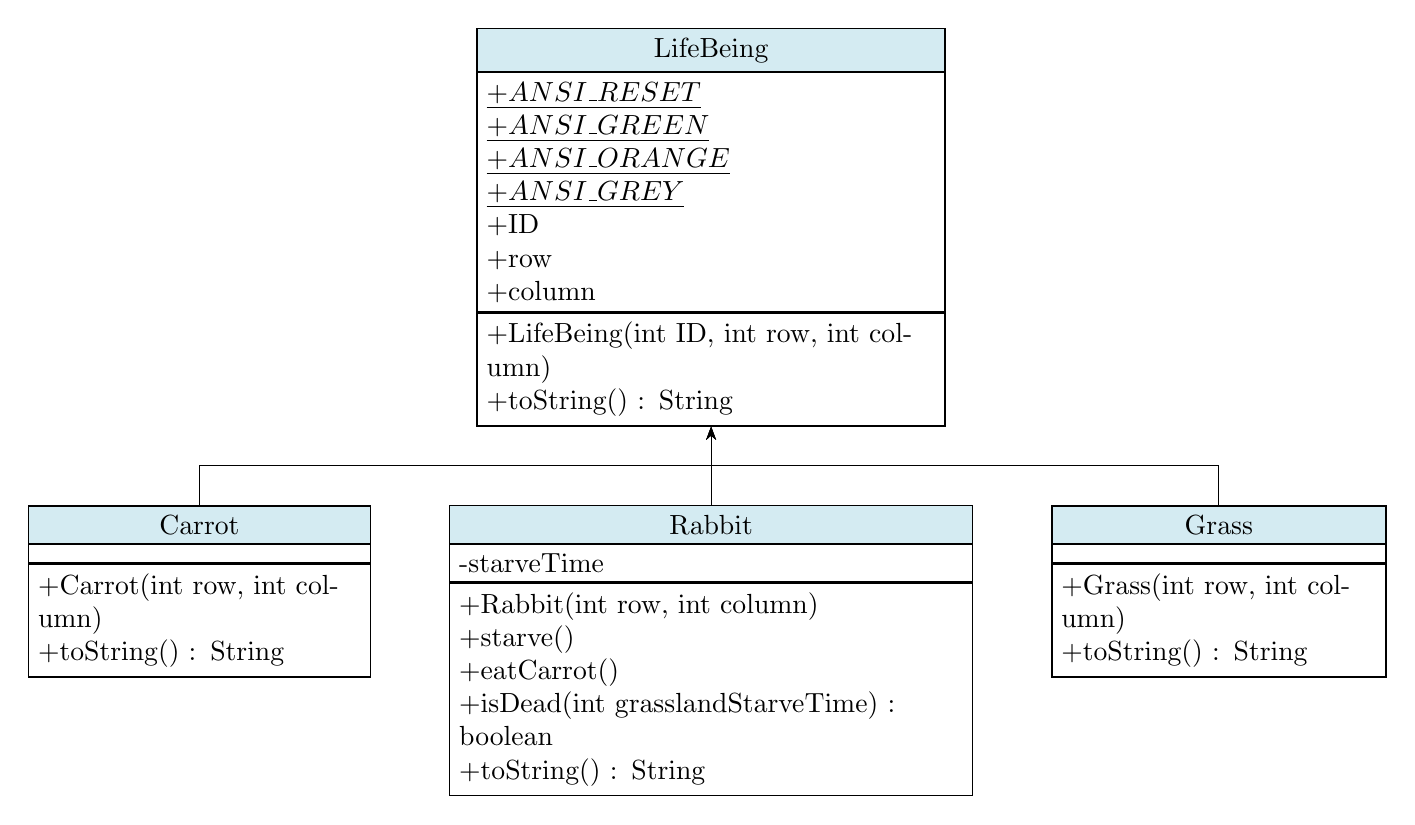
\begin{tikzpicture}[>=Stealth]

    % --- Begin Life Being Node ---
			\node [draw, rectangle, text width=5.7cm, align=center, fill=light_blue] (LifeBeing) {LifeBeing};
			\node [draw, rectangle, text width=5.7cm, below=0.0cm of LifeBeing, align=left] (life_being_attributes) {
				\(\underline{+ANSI\_RESET}\) \\
				\(\underline{+ANSI\_GREEN}\) \\
				\(\underline{+ANSI\_ORANGE}\) \\
				\(\underline{+ANSI\_GREY}\) \\
				+ID \\
				+row \\
				+column \\
			};
			\node [draw, rectangle, text width=5.7cm, below=0.0cm of life_being_attributes, align=left] (life_being_methods) {
				+LifeBeing(int ID, int row, int column) \\
				+toString() : String
			};
    
			% Merge all the nodes so it can turn all this nodes into one.
			\node [draw, fit={(LifeBeing) (life_being_attributes) (life_being_methods)}, inner sep=0pt] (LifeBeingNode) {};
			% --- End Life Being Node ---

			% -- Begin Rabbit Node. ---
			\node [draw, rectangle, below=of LifeBeingNode, text width=6.4cm, align=center, fill=light_blue] (Rabbit) {Rabbit};
			\node [draw, rectangle, text width=6.4cm, below=0.0cm of Rabbit, align=left] (rabbit_attributes) {
				-starveTime
			};
			\node [draw, rectangle, text width=6.4cm, below=0.0cm of rabbit_attributes, align=left] (rabbit_methods) {
				+Rabbit(int row, int column) \\
				+starve() \\
				+eatCarrot() \\
				+isDead(int grasslandStarveTime) : boolean \\
				+toString() : String
			};

			% Merge Rabbit Nodes.
			\node [draw, fit={(Rabbit) (rabbit_attributes) (rabbit_methods)}, inner sep=0pt] (RabbitNode) {};
			% --- End Rabbit Node. ---

			% --- Begin Carrot Node. ---
			\node [draw, rectangle, left=of Rabbit, text width=4.1cm, align=center, fill=light_blue] (Carrot) {Carrot};
			\node [draw, rectangle, text width=4.1cm, below=0.0cm of Carrot, align=left] (carrot_attributes) {};
			\node [draw, rectangle, text width=4.1cm, below=0.0cm of carrot_attributes, align=left] (carrot_methods) {
				+Carrot(int row, int column) \\
				+toString() : String
			};

			% Merge Carrot Nodes.
			\node [draw, fit={(Carrot) (carrot_attributes) (carrot_methods)}, inner sep=0pt] (CarrotNode) {};
			% --- End Carrot Node. ---

			% --- Begin Grass Node. ---
			\node [draw, rectangle, right=of Rabbit, text width=4.0cm, align=center, fill=light_blue] (Grass) {Grass};
			\node [draw, rectangle, text width=4.0cm, below=0.0cm of Grass, align=left] (grass_attributes) {};
			\node [draw, rectangle, text width=4.0cm, below=0.0cm of grass_attributes, align=left] (grass_methods) {
				+Grass(int row, int column) \\
				+toString() : String
			};

			% Merge Grass Nodes.
			\node [draw, fit={(Grass) (grass_attributes) (grass_methods)}, inner sep=0pt] (GrassNode) {};
			% --- End Grass Node. ---

			% Connect the nodes.
			\draw[->] (RabbitNode.north) -- ++(0,0.5) -| (LifeBeingNode.south);
			\draw[->] (CarrotNode.north) -- ++(0,0.5) -| (LifeBeingNode.south);
			\draw[->] (GrassNode.north) -- ++(0,0.5) -| (LifeBeingNode.south);

  \end{tikzpicture}
  \caption{Diagrama de classes}
\end{figure}
\clearpage % Forces all figures above it in the .tex file to be printed before continuing with the text. This can leave large white spaces. More info in https://tex.stackexchange.com/questions/8625/force-figure-placement-in-text

\begin{figure}[h]
	\hspace{-2.5cm} % Move whole figure 2.5cm to the left.
	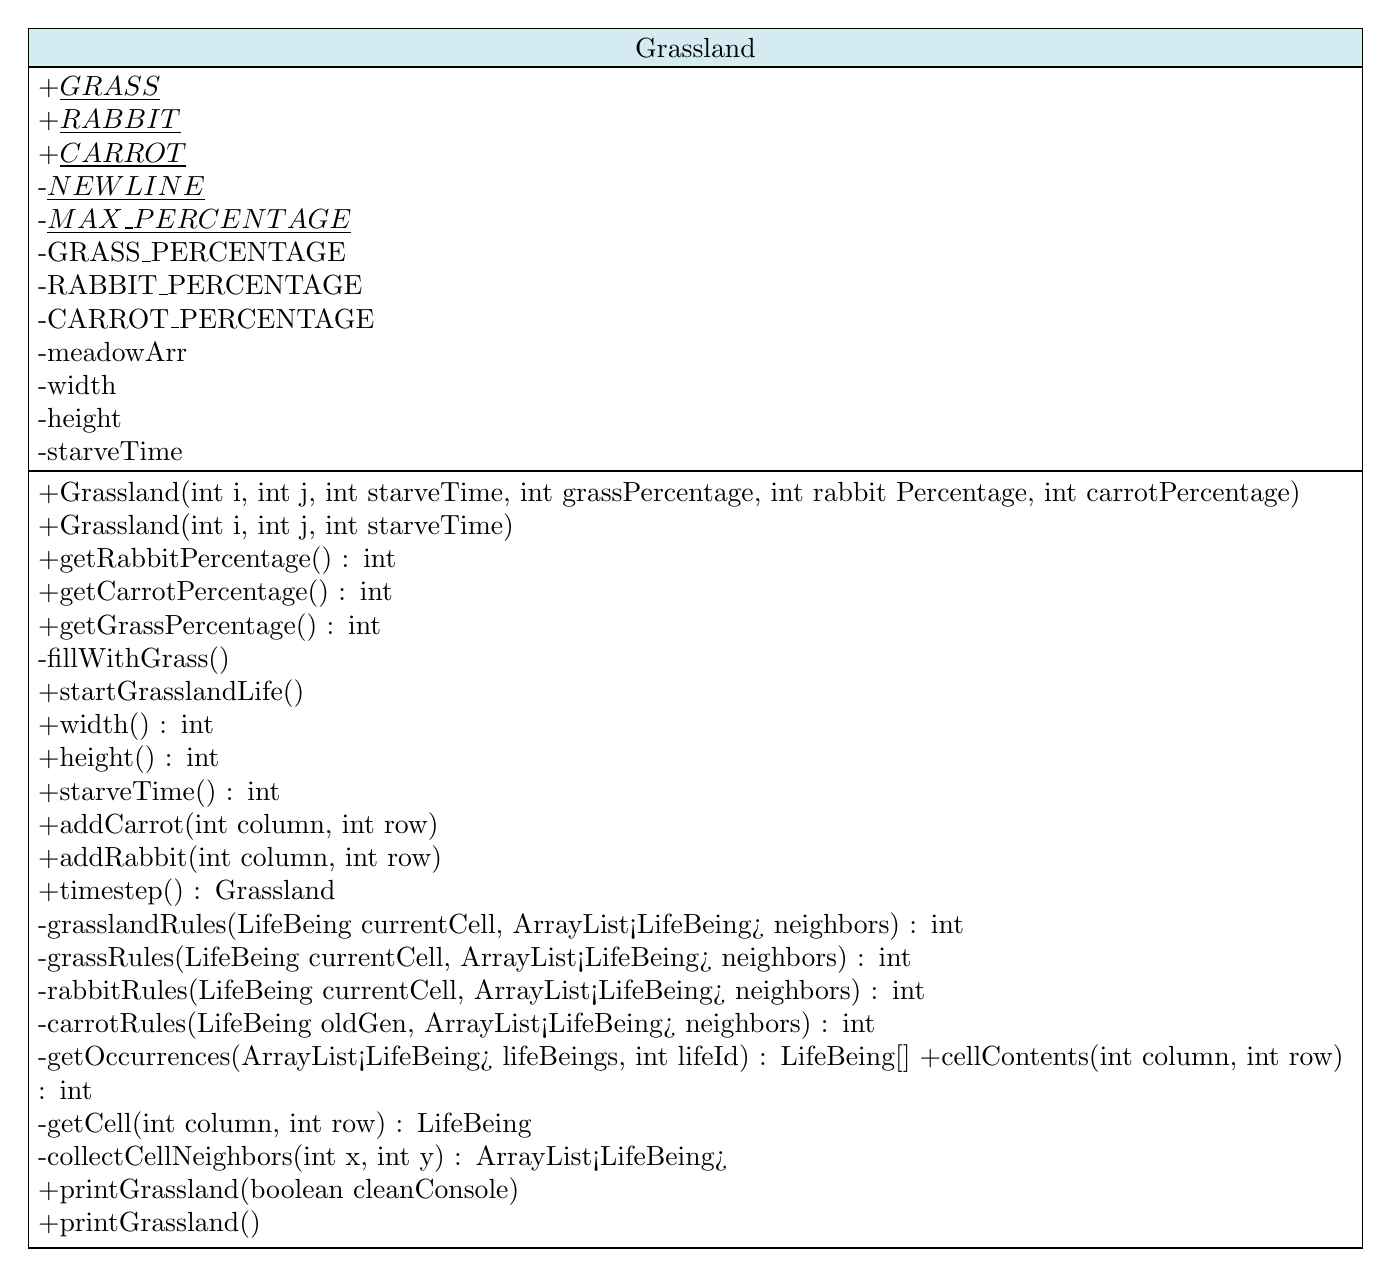
\begin{tikzpicture}
			% --- Begin Grassland Node ---
			\node [draw, rectangle, text width=16.7cm, align=center, fill=light_blue] (Grassland) {Grassland};
			\node [draw, rectangle, text width=16.7cm, below= 0.0cm of Grassland, align=left] (grassland_attributes) {
				+\(\underline{GRASS}\) \\
				+\(\underline{RABBIT}\) \\
				+\(\underline{CARROT}\) \\
				-\(\underline{NEWLINE}\) \\
				-\(\underline{MAX\_PERCENTAGE}\) \\
				-GRASS\_PERCENTAGE \\
				-RABBIT\_PERCENTAGE \\
				-CARROT\_PERCENTAGE \\
				-meadowArr \\
				-width \\
				-height \\
				-starveTime \\
			};
			\node [draw, rectangle, text width=16.7cm, below=0.0cm of grassland_attributes, align=left] (grassland_methods) {
				+Grassland(int i, int j, int starveTime, int grassPercentage, 
									 int rabbit Percentage, int carrotPercentage) \\
				+Grassland(int i, int j, int starveTime) \\
				+getRabbitPercentage() : int \\
				+getCarrotPercentage() : int \\
				+getGrassPercentage() : int \\
				-fillWithGrass() \\
				+startGrasslandLife() \\
				+width() : int \\
				+height() : int \\
				+starveTime() : int \\
				+addCarrot(int column, int row) \\
				+addRabbit(int column, int row) \\
				+timestep() : Grassland \\
				-grasslandRules(LifeBeing currentCell, ArrayList<LifeBeing> neighbors) : int \\
				-grassRules(LifeBeing currentCell, ArrayList<LifeBeing> neighbors) : int \\
				-rabbitRules(LifeBeing currentCell, ArrayList<LifeBeing> neighbors) : int \\
				-carrotRules(LifeBeing oldGen, ArrayList<LifeBeing> neighbors) : int \\
				-getOccurrences(ArrayList<LifeBeing> lifeBeings, int lifeId) : LifeBeing[]
				+cellContents(int column, int row) : int \\
				-getCell(int column, int row) : LifeBeing \\
				-collectCellNeighbors(int x, int y) : ArrayList<LifeBeing> \\ 
				+printGrassland(boolean cleanConsole) \\
				+printGrassland()
			};
			
			% Merge all the nodes so it can turn all this nodes into one.
			\node [draw, fit={(Grassland) (grassland_attributes) (grassland_methods)}, inner sep=0pt] (GrasslandNode) {};
			% --- End Grassland Node ---
		\end{tikzpicture}
		\caption{Diagrama de classes}
	\end{figure}
\clearpage

\subsection{Execução}	
	\begin{minted}[autogobble, tabsize=2, obeytabs]{shell-session}
		javac life_beings/*.java && javac exceptions/*.java && javac main/*.java && java main.Main 
	\end{minted}

\subsection{Output}
	Os resultados podem ser visíveis de duas formas:
	\begin{enumerate}
		\item Na linha de comandos, permitindo a execução do método de instância 
		   		\textit{printGrassland()} no método \textit{startGrasslandLife()}.
		\item Numa janela que surge no meio do monitor.
	\end{enumerate}

\section{Conclusão}
	Em suma, as principais dificuldades foram mitigadas aplicando os resultados 
	das regras diretamente no prado (\textit{Grassland}) instanciado, 
	e o objetivo foi cumprido, havendo resultados visíveis da aplicação das regras 
	da vida. 

	Além disso, concluiu-se que o paradigma da POO é especialmente útil 
	para representar problemas de uma forma mais natural a como os vemos,
	com objetos com várias partes que interagem entre si.

	Pode-se referir, por último, que regras simples demonstraram ser capazes 
	de gerar padrões complexos, o que criou um elo de ligação entre o 
	(quase antagónico) determinismo da tecnologia e a imprevisível natureza da vida.

\end {document}
